% --------------------------------------------------------------
% This is all preamble stuff that you don't have to worry about.
% Head down to where it says "Start here"
% --------------------------------------------------------------
 
\documentclass[12pt]{article}
 
\usepackage[margin=1in]{geometry} 
\usepackage{amsmath,amsthm,amssymb}
\usepackage{graphicx}
\graphicspath{{./images}}
 
\newcommand{\N}{\mathbb{N}}
\newcommand{\Z}{\mathbb{Z}}
 
\newenvironment{theorem}[2][Theorem]{\begin{trivlist}
\item[\hskip \labelsep {\bfseries #1}\hskip \labelsep {\bfseries #2.}]}{\end{trivlist}}
\newenvironment{lemma}[2][Lemma]{\begin{trivlist}
\item[\hskip \labelsep {\bfseries #1}\hskip \labelsep {\bfseries #2.}]}{\end{trivlist}}
\newenvironment{exercise}[2][Exercise]{\begin{trivlist}
\item[\hskip \labelsep {\bfseries #1}\hskip \labelsep {\bfseries #2.}]}{\end{trivlist}}
\newenvironment{reflection}[2][Reflection]{\begin{trivlist}
\item[\hskip \labelsep {\bfseries #1}\hskip \labelsep {\bfseries #2.}]}{\end{trivlist}}
\newenvironment{proposition}[2][Proposition]{\begin{trivlist}
\item[\hskip \labelsep {\bfseries #1}\hskip \labelsep {\bfseries #2.}]}{\end{trivlist}}
\newenvironment{corollary}[2][Corollary]{\begin{trivlist}
\item[\hskip \labelsep {\bfseries #1}\hskip \labelsep {\bfseries #2.}]}{\end{trivlist}}


\newenvironment{sol}[1][Solution]{\begin{trivlist}
\item[\hskip\labelsep {\bfseries #1:}]}{\end{trivlist}}
\begin{document}
 
% --------------------------------------------------------------
%                         Start here
% --------------------------------------------------------------
 
\renewcommand{\qedsymbol}{\filledbox}
\begin{center}
    CSE 5/7350 Quiz 1 \\
Background Material \\
%replace X with the appropriate number
January 17, 2023\\
\end{center}

\begin{flushright}
Name: Bingying Liang\\  %replace with your name
ID: 48999397
\end{flushright}
  %if necessary, replace with your course title

% \title{CSE 5/7350 Quiz 1 \\
% Background Material \\
% }%replace X with the appropriate number
% \date{January 17, 2023}

% \author{ 
% Name: Bingying Liang \\ %replace with your name
% ID: 48999397\\
%  } %if necessary, replace with your course title

% \maketitle

\textbf{All Questions are 4 points each:}\\
\begin{enumerate}
    % 1
    \item Find a simple formula for $\sum_{i=1}^k(2i-1)$
    \begin{sol}
        \begin{align*}
    \sum_{i=1}^k(2i-1) & = (2 \times 1 -1) + (2 \times 2-1)+(2 \times 3 -1) + \dots + (2 \times k -1)\\
    & = (2 \times 1) + (2 \times 2) + (2 \times 3) + \dots + 2k  - k\\
    & = 2(\frac{(1+k)k}{2}-k) \\
    & = k(1+k-1) \\
    & = k^2
\end{align*}
    \end{sol}

    %2
    \item Find a simple formula for $\sum_{i=1}^k(3+i^2)$
    \begin{sol}
        \begin{align*}
        \sum_{i=1}^k(3+i^2) = \sum_{i=1}^k3 +\sum_{i=1}^k i^2= 3k + \sum_{i = 1}^k i^2 
        \end{align*}
        \begin{align*}
        \because \sum_{i=1}^k[(i+1)^3 - i^3] &= \sum_{i=1}^k[(i^3+3i^2+3i+1)-i^3] \\
        &= \sum_{i=1}^k(3i^2 + 3i +1) \\
        &= 3\sum_{i=1}^ki^2 + 3\sum_{i=1}^ki + \sum_{i=1}^k 1 \\
        &= 3 \sum_{i=1}^ki^2 + 3\frac{(1+k)k}{2}+k\\
        \end{align*}
        \begin{align*}
            \because \sum_{i=1}^k[(i+1)^3 - i^3] &=[(1+1)^3-1^3]+[(2+1)^3-2^3]+[(3+1)^3-3^3]+\dots+[(k+1)^3 - k^3] \\
            & = (2^3 -1^3) +(3^3-2^3)+(4^3-3^3)+\dots+[(k+1)^3 - k^3]\\
            & = -1^3+(k+1)^3 
        \end{align*}
        \begin{align*}
            \therefore -1^3+(k+1)^3 &= 3 \sum_{i=1}^ki^2 + 3\frac{(1+k)k}{2}+k \\
            3\sum_{i=1}^ki^2&=(k+1)^3-1-3\frac{(1+k)k}{2}-k \\
            \sum_{i=1}^ki^2& = \frac{2(k+1)^3-2(k+1)-3(k+1)k}{6}\\
            \sum_{i=1}^ki^2&= \frac{(k+1)[2(k+1)^2-2-3k)]}{6}\\
            \sum_{i=1}^ki^2&= \frac{(k+1)[2(k^2+2k+1)-2-3k]}{6}\\
            \sum_{i=1}^ki^2&= \frac{(k+1)(2k^2+k)}{6}\\
            \sum_{i=1}^ki^2&= \frac{k(k+1)(2k+1)}{6}
        \end{align*}
        \begin{align*}
             \sum_{i=1}^k(3+i^2) = 3k+\frac{k(k+1)(2k+1)}{6}
        \end{align*}
    \end{sol}

    %3
    \item Compute the value of $\sum_{i = 1}^{\infty}(\frac{1}{2})^{i-1}$
    \begin{sol}
    \begin{align*}
    \sum_{i=1}^{\infty}(\frac{1}{2})^{i-1}
    & = \lim_{n \rightarrow{\infty}}[(\frac{1}{2})^0 + (\frac{1}{2})^1 (\frac{1}{2})^3 + \dots + (\frac{1}{2})^n] \\
    & = \lim_{n \rightarrow{\infty}}[\frac{1(1-(\frac{1}{2})^n)}{1-\frac{1}{2}}] \\
    & = \lim_{n \rightarrow{\infty}}\frac{1-\frac{1}{2^n}}{\frac{1}{2}}\\
    & = \frac{1-0}{\frac{1}{2}}\\
    & = 2
\end{align*}
    \end{sol}

    %4
    \item Compute the value of $  \lim\limits_{n\to\infty} (\frac{4n}{3n})$
    \begin{sol}
    \begin{align*}
    \lim_{n \to \infty}(\frac{4n}{3n})= \lim_{n \to \infty}{\frac{4}{3}} = \frac{4}{3}
\end{align*}
    \end{sol}

    
    %5
    \item Compute the value of $\lim\limits_{n \to \infty}(\frac{n^4}{n^3})$
    \begin{sol}
        \begin{align*}
            \lim_{n \to \infty}(\frac{n^4}{n^3}) 
            = \lim_{n \to \infty}\frac{\frac{n^4}{n^3}}{\frac{n^3}{n^3}} 
            = \lim_{n \to \infty} \frac{n}{1} = \infty
        \end{align*}
    \end{sol}

    %6
    \item Compute the value of $\lim\limits_{n \to \infty}(\frac{2^n}{5^n})$
    \begin{sol}
        \begin{align*}
            \lim_{n \to \infty}(\frac{2^n}{5^n})
            = \lim_{n \to \infty}(\frac{2}{5})^n = 0 
        \end{align*}
    \end{sol}

    %7
    \item Compute the value of $\lim\limits_{n \to \infty}(\frac{n!}{(n+2)!})$
    \begin{sol}
        \begin{align*}
            \lim_{n \to \infty}(\frac{n!}{(n+2)!}) 
            = \lim_{n \to \infty}{\frac{n!}{n!(n+1)(n+2)}} 
            = \lim_{n \to \infty}{\frac{1}{(n+1)(n+2)}}
            = 0
        \end{align*}
    \end{sol}

    %8
    \item Compute the value of $\lim\limits_{n \to \infty}(\frac{\log_{12}n}{\log_3n})$
    \begin{sol}
        \begin{align*}
            \lim\limits_{n \to \infty}(\frac{\log_{12}n}{\log_3n})
            = \lim\limits_{n \to \infty}\frac{\frac{\log_3n}{\log_3 12}}{\log_3 n}
            = \lim_{n \to \infty}\frac{1}{\log_3 12} = \frac{1}{\log_3 12}
        \end{align*}
    \end{sol}

    %9
    \item Compute $\log_2 487$. Give your answer rounded to 6 decimal places (x.xxxxxx)
    \begin{sol}
        \begin{align*}
        \log_{2}487 \approx 8.9277778
        \end{align*}
    \end{sol}

~\\

Consider a bag of 7 blocks. Each block has a different color. The colors are Red, Orange,Yellow, Green, Blue, Indigo and Violet.

    %10
    \item How many different ways can you pick out 4 blocks from a bag of 7 blocks? The order you pick out the blocks does not matter. (answer with an integer)
    \begin{sol}
        \begin{align*}
            C_7^4 = \frac{7!}{4!(7-4)!} = \frac{7!}{4!3!}=\frac{7\times 6\times 5\times 4!}{4! 3!}=\frac{7\times6\times5}{6} = 35 
        \end{align*}
    \end{sol}

    %11
    \item How many different ways can you rearrange the 7 blocks? (answer with an integer)
    \begin{sol}
        \begin{align*}
            7!=7\times6\time5\times4\times3\times2\times1 = 5040
        \end{align*}
    \end{sol}

    %12 
    \item You reach into the bag and pull out a block. What is the probability that it is Red, Orange or Yellow or Green and not Blue, Indigo or Violet?
    \begin{sol}
        \begin{align*}
            P=P(Red)+P(Orange)+P(Yellow)+P(Green)=\frac{1}{7} + \frac{1}{7} + \frac{1}{7} +\frac{1}{7} = \frac{4}{7}
        \end{align*}
    \end{sol}

    %13
    \item You reach into the bag of 7 blocks and pull out 2 blocks. What is the probability that at least one of the blocks you pulled out is Red, or Orange?
    \begin{sol}
        \begin{align*}
        P = 1 - P(None \ of \ Red \ or \ Orange) = 1- \frac{5}{7} \times \frac{4}{6}=1-\frac{20}{42} = \frac{42-20}{42} = \frac{22}{42} = \frac{11}{21}
        \end{align*}
    \end{sol}
~\\


\leftline {\textbf{Answer the following questions with either:\\}}
A. The time depends on size of n and twice as large will likely require about twice the time.\\
B. The time depends on size of n but twice as large will generally be less than twice the time.\\
C. Constant amount of time regardless of size of n\\



    %14
    \item How long will it take to insert an element at the head of a linked list of size n?
    \begin{sol}
        \begin{align*}
        C
        \end{align*}
    \end{sol}

    

    %15
    \item How long will it take to remove an element from a doubly linked list of size n if you only have a pointer to the element you wish to remove and are unable to copy the data of the elements?
    \begin{sol}
        \begin{align*}
            C
        \end{align*}
    \end{sol}


    %16
    \item How long will it take to remove an element from a linked list of size n if you only have a pointer to the element you wish to remove?
    \begin{sol}
        \begin{align*}
        C
        \end{align*}
    \end{sol}

    %17
    \item How long will it take to insert an element at the beginning of an array of size n?
    \begin{sol}
        \begin{align*}
        A
        \end{align*}
    \end{sol}

    %18
    \item How long will it take to delete element k (where k is close to 1/2 n) from an array of size n where order does not matter?
    \begin{sol}
        \begin{align*}
        A
        \end{align*}
    \end{sol}
    
    %19
    \item How long will it take to delete element k (where k is close to 1/2 n) from an array of size n where order does matter?
    \begin{sol}
        \begin{align*}
        A
        \end{align*}
    \end{sol}
    
    %20
    \item How long will it take to determine if an element exists in a sorted linked list of size n?
    \begin{sol}
        \begin{align*}
        A
        \end{align*}
    \end{sol}
    
    %21
    \item How long will it take to determine if an integer exists in a sorted array of n integers?
    \begin{sol}
        \begin{align*}
        B
        \end{align*}
    \end{sol}

    %22
    \item How long will it take to correctly insert an element into an AVL tree of size n.
    \begin{sol}
        \begin{align*}
        B
        \end{align*}
    \end{sol}

Consider the following tree:\\
    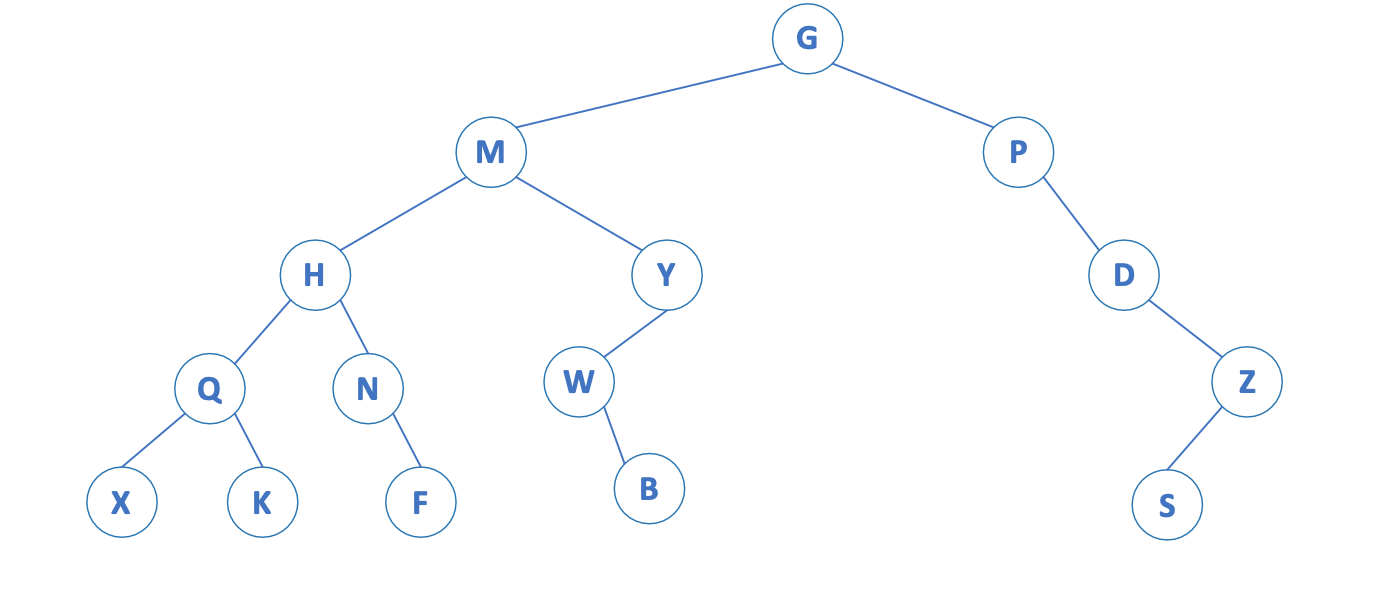
\includegraphics[width=0.9\textwidth]{image.png}

    %23
    \item Give a pre-order traversal of the tree
    \begin{sol}
        \begin{align*}
            G, M, H, Q, X, K, N, F, Y, W, B, P, D, Z, S
        \end{align*}
    \end{sol}
    
    %24
    \item Give a post-order traversal of the tree
    \begin{sol}
        \begin{align*}
            X, K, Q, F, N, H, B, W, Y, M, S, Z, D, P, G
        \end{align*}
    \end{sol}

    %25
    \item Give a in-order traversal of the tree
    \begin{sol}
        \begin{align*}
            X, Q, K, H, N, F, M, W, B, Y, G, P, D, S, Z
        \end{align*}
    \end{sol}
    
    
\end{enumerate}







% \begin{exercise}{1} %You can use theorem, proposition, exercise, or reflection here.  Modify x.yz to be whatever number you are proving
% $f(x)$ is given by formula: 
% \end{exercise}
 
% \begin{exercise}
% 1We are finding limits by using the "plug-in method" for numbers approaching 3 from the right :
% %Note 1: The * tells LaTeX not to number the lines.  If you remove the *, be sure to remove it below, too.
% %Note 2: Inside the align environment, you do not want to use $-signs.  The reason for this is that this is already a math environment. This is why we have to include \text{} around any text inside the align environment.
% \begin{align*}
% \lim_{x \to 3^+} (x^2+2) &= ?  \\
% &  \text{Consider for }"x":  3.1,
%                3.01,
%                3.001,
%                3.0001\text{} \\
% & \lim(3.1^2+2)=11.61\\
% & \lim(3.01^2+2)=11.0601\\
% & \lim(3.001^2+2)=11.006001 \\
% & \lim(3.0001^2+2)=11.0006
% \end{align*}
% \end{exercise}
 
% \begin{proposition}{}
% $\lim_{x \to 3^+} (x^2+2)$
% Let $x=11$. 
% \end{proposition}
 
% \begin{proof}%Whatever you put in the square brackets will be the label for the block of text to follow in the proof environment.
% Since all of the outcomes just keep getting closer to 11 one can assume that the limit as "x" approaches 3 from the right the limit will be equal to 11.
% % * <arking4@g.coastal.edu> 2015-08-24T22:28:35.113Z:
% %
% % 
% %
% \end{proof}
 
% --------------------------------------------------------------
%     You don't have to mess with anything below this line.
% --------------------------------------------------------------
 
\end{document}